\documentclass{article}
\usepackage{tikz}
\usetikzlibrary{arrows.meta,positioning,calc,shapes.geometric}
\pagestyle{empty}
\begin{document}
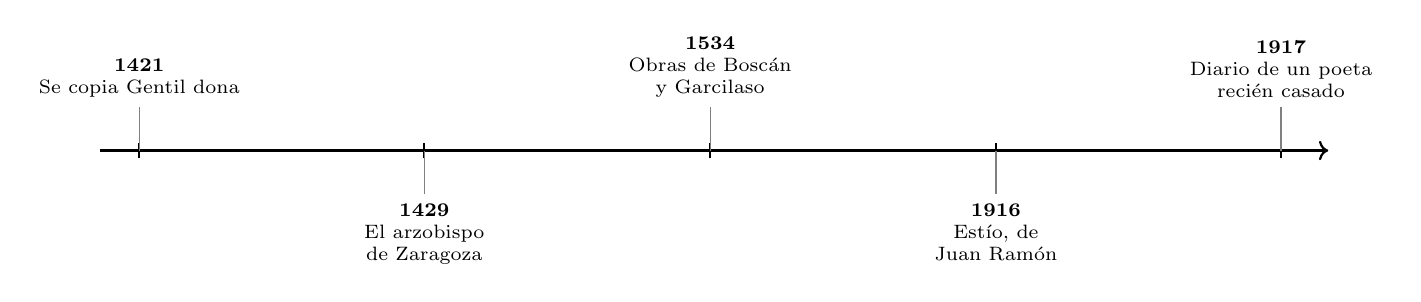
\begin{tikzpicture}
\tikzset{every node/.append style={align=center}}
\draw[->, thick] (-0.5,0) -- (15.10,0);
\draw[thick] (0.00,-0.1) -- (0.00,0.1);
\draw[gray] (0.00,0) -- (0.00,0.55);
\node[anchor=south, align=center, text width=2.60cm, font=\scriptsize] at (0.00,0.55) {\textbf{1421}\\ Se copia Gentil dona};
\draw[thick] (3.62,-0.1) -- (3.62,0.1);
\draw[gray] (3.62,0) -- (3.62,-0.55);
\node[anchor=north, align=center, text width=2.60cm, font=\scriptsize] at (3.62,-0.55) {\textbf{1429}\\ El arzobispo de Zaragoza};
\draw[thick] (7.25,-0.1) -- (7.25,0.1);
\draw[gray] (7.25,0) -- (7.25,0.55);
\node[anchor=south, align=center, text width=2.60cm, font=\scriptsize] at (7.25,0.55) {\textbf{1534}\\ Obras de Boscán y Garcilaso};
\draw[thick] (10.88,-0.1) -- (10.88,0.1);
\draw[gray] (10.88,0) -- (10.88,-0.55);
\node[anchor=north, align=center, text width=2.60cm, font=\scriptsize] at (10.88,-0.55) {\textbf{1916}\\ Estío, de Juan Ramón};
\draw[thick] (14.50,-0.1) -- (14.50,0.1);
\draw[gray] (14.50,0) -- (14.50,0.55);
\node[anchor=south, align=center, text width=2.60cm, font=\scriptsize] at (14.50,0.55) {\textbf{1917}\\ Diario de un poeta recién casado};
\end{tikzpicture}
\end{document}
